\documentclass[a4paper,oneside,10pt]{article}
\usepackage[spanish]{babel} % Idioma
\usepackage[utf8x] {inputenc} % Codificación
\usepackage {comment} % Permite utilizar el entorno comment
\usepackage {amsmath} % Cosas de matemática
\pagestyle {plain} % Configuración de página
\usepackage{graphicx} % Gráficos
\usepackage{titling}
\newcommand{\subtitle}[1]{%
  \posttitle{%
    \par\end{center}
    \begin{center}\large#1\end{center}
    \vskip0.5em}%
}
\usepackage{setspace}
\usepackage[T1]{fontenc}
\usepackage{float}
\usepackage{subcaption}
\usepackage{amsmath}
\usepackage{graphicx}
\usepackage[colorinlistoftodos]{todonotes}
\usepackage[colorlinks=true, allcolors=blue]{hyperref}
\usepackage{fancyhdr}
\pagestyle{fancy}
\usepackage{caption}
\usepackage{mathtools}
\usepackage{booktabs}
\usepackage{indentfirst}
\usepackage{enumitem}
\usepackage{siunitx}
\begin {document}

\begin{titlepage}
\thispagestyle{empty}

\begin{center}

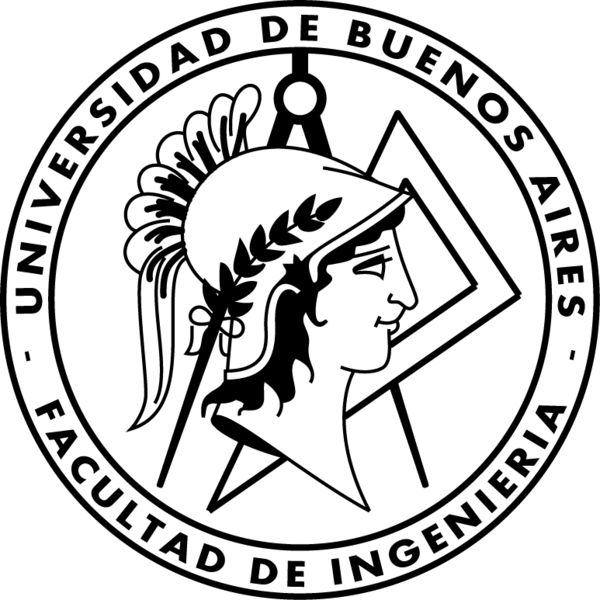
\includegraphics[scale=1.2]{Imagenes/Logo_Fiuba2.png}

\bigskip
\textbf{UNIVERSIDAD DE BUENOS AIRES}

\smallskip

\textbf{Facultad de Ingeniería}

\smallskip

\textbf{Departamento de Electrónica}

\vspace{2cm}

\textbf{\Large{Sistemas Irradiantes (86.29)}}

\vspace{1cm}

\textbf{\large{Lineas De Transmisión}}

\vspace{0.5cm}

\textbf{\large{Guía 1}}

\vspace{1cm}

\today

\vspace{1cm}

\begin{tabular}{lcl}
SAMBRIZZI, Matias & \ \ \ 98531 & \ \ \ 
\texttt{\href{mailto:msambrizzi@fi.uba.ar}{msambrizzi@fi.uba.ar}}\\
\end{tabular}

\end {center}

\end{titlepage}
\newpage
\pagestyle{fancy}
\lhead{Sistemas Irradiantes (86.29)}
%\rhead{\nouppercase{\leftmark}}
\rhead{Lineas de transmisión}


\spacing{1.5}

\section{}



\end{document}